\documentclass[11pt]{article}
\usepackage[utf8]{inputenc} % Para caracteres en espa�ol
\usepackage{amsmath,amsthm,amsfonts,amssymb,amscd}
\usepackage{multirow,booktabs}
\usepackage[table]{xcolor}
\usepackage{fullpage}
\usepackage{lastpage}
\usepackage{enumitem}
\usepackage{floatrow}
\usepackage{multicol}
\usepackage{fancyhdr}
\usepackage{mathrsfs}
\usepackage{wrapfig}
\usepackage[final]{pdfpages}
\usepackage{setspace}
\usepackage{esvect}
\usepackage{calc}
\usepackage{multicol}
\usepackage{cancel}
\usepackage{graphicx}
\graphicspath{ {picturesB/} }
\usepackage[retainorgcmds]{IEEEtrantools}
\usepackage[margin=3cm]{geometry}
\usepackage{amsmath}
\newlength{\tabcont}
\setlength{\parindent}{0.0in}
\setlength{\parskip}{0.05in}
\usepackage{empheq}
\usepackage{framed}
%\usepackage{newtxmath}
\usepackage{euscript}
\DeclareMathAlphabet{\mathpzc}{T1}{pzc}{m}{it}
\usepackage[most]{tcolorbox}
\usepackage{xcolor}
\colorlet{shadecolor}{orange!15}
\parindent 0in
\parskip 12pt
\geometry{margin=1in, headsep=0.25in}
\theoremstyle{definition}
\newtheorem{defn}{Definition}
\newtheorem{reg}{Rule}
\newtheorem{exer}{Exercise}
\newtheorem{note}{Note}
\newcommand{\volume}{{\ooalign{\hfil$V$\hfil\cr\kern0.08em--\hfil\cr}}}
\newcommand{\parr}{\mathbin{\|}} % Parralel Symbol
\begin{document}
\setcounter{section}{2}%Section we want -1
\setcounter{page}{24} %Page we want
\setcounter{equation}{78}%Equation we want -1
\def\thepart{\arabic{part}}
\setcounter{part}{9}
\numberwithin{equation}{part}

 \pagestyle{fancy}
\fancyhf{}
\rhead{Section 9:  Electrostatic Propulsion - Electrospray/Colloid Thrusters}
\rfoot{Page \thepage}
\thispagestyle{empty}

\begin{center}
{\LARGE \bf Section 9:  Electrostatic Propulsion}\\
{\large AE435}\\
Spring 2018
\end{center}
\vspace{5mm}
\section{Electrospray/Colloid Thrusters}
\vspace{25mm}
\tableofcontents
\newpage
Electrospray/colloid propulsion different from ion thruster and HET, but still electrostatic propulsion.  Main difference = liquid propellant, not noble gas (xenon).
 
In electrospray/colloid propulsion charged particles are extracted from a liquid and accelerated to high speed.  These particles are generally not individual atoms (not Xe+ or Li+), but are typically molecular species (e.g., 1-Ethyl-3-methylimidazolium a.k.a. Emim+ or BF4-  tetrafluoroborate) and cluster/droplets of those species (e.g., many hundreds of molecules bonded together within a droplet, which likely has charge-state >1)
 
Three main types of technologies, based on the type of liquids and type of emission:
\begin{enumerate}
\item Colloid thruster - accelerates and expels charged droplets, and uses solvents such as glycerol and formamide as propellant
\item Field emission electric propulsion (FEEP) - uses liquid metals (Cs and In) to emit positively charged metal ions
\item Ionic liquid ion sources (ILIS) - room-temperature molten salts (i.e., "ionic liquids") used to create ion beams (individual molecular ion emission) or mixtures of ions with droplets.  No need to ionize, free charges already present in the liquid.
 \end{enumerate}
Electrospray well-known in chemistry and materials analysis community.  Electrospray ionization used in mass spectrum analysis to study liquids.  Ions/droplets extracted from liquid and mass spectrum analyzed, usually for bio-related materials, e.g., proteins, prescription drugs.
 
  \begin{center}
{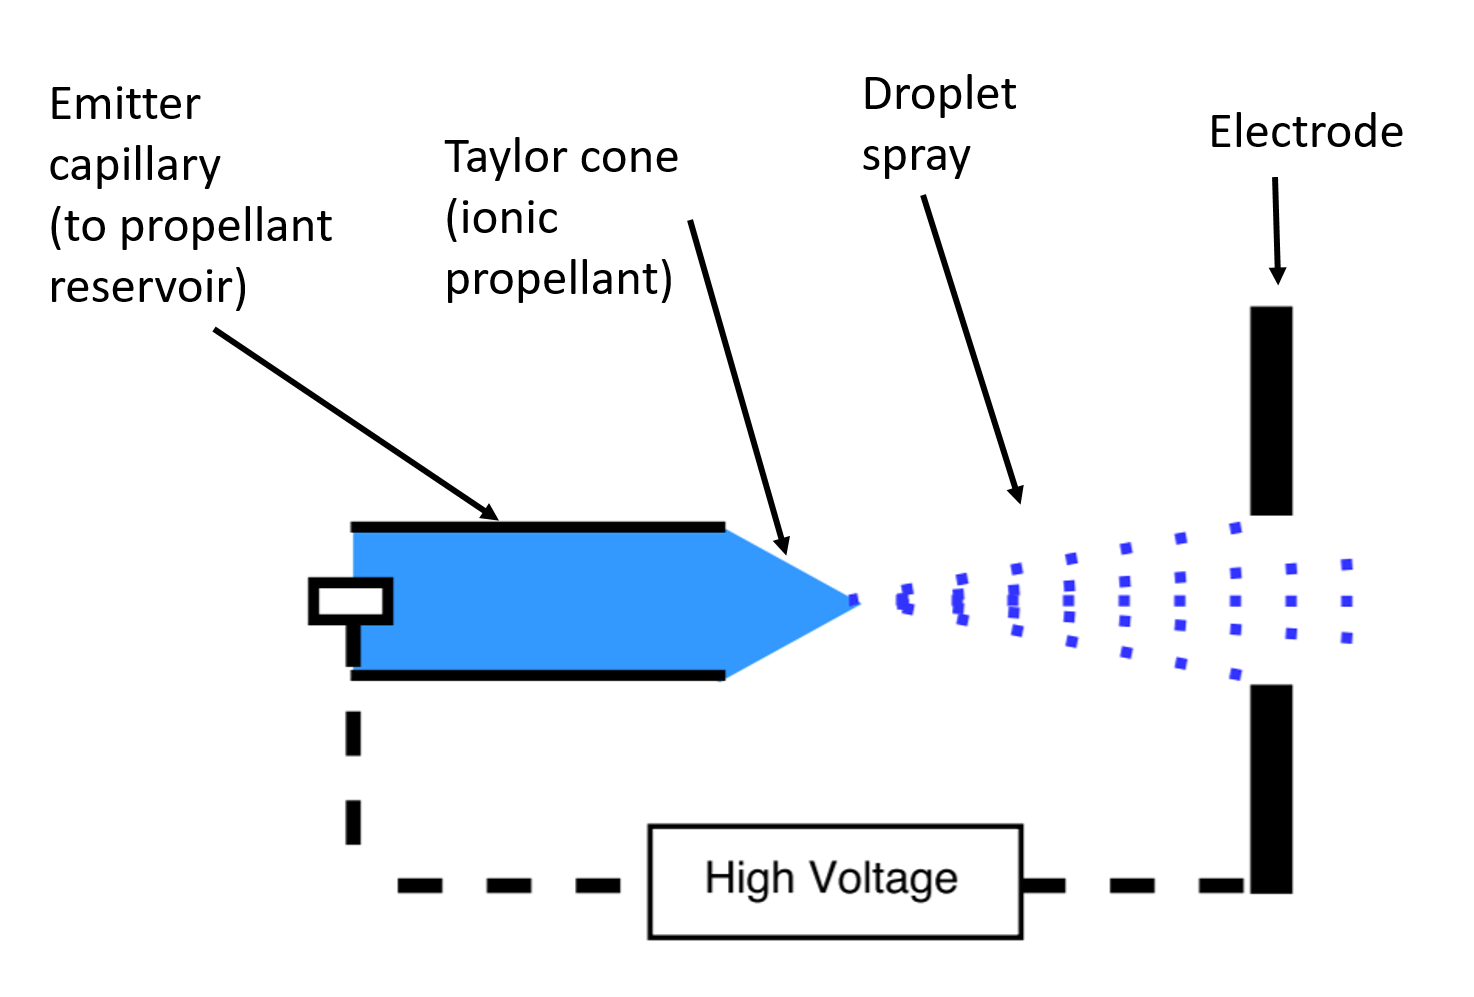
\includegraphics[scale=0.5]{31.png}}
\end{center}
%These propellants can conduct adnw e are extrating out the ions at the tip. , being accelerated by the electric field. The m
 \begin{center}
{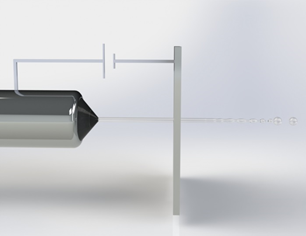
\includegraphics[scale=0.5]{32.png}}
\end{center}

Motivation for electrospray propulsion
%Samll packaging, possibly better efficiency becasue you dont have to pay any ionization cost. 
High thrust-density.
Remember

Converting electric potential to kinetic energy. 
   \begin{equation}
 \begin{aligned}
 q \, V_{acc} = \frac{1}{2} Mv^2 \quad \rightarrow \quad V_{accel} = \frac{Mv^2}{2q}
 \end{aligned}
 \end{equation}
 
Thrust can be written as ...
   \begin{equation*}
 \begin{aligned}
 T = \dot{m}_i \, v_i = \frac{I_bM}{e} \, \sqrt{\frac{2eV}{M}} 
 \end{aligned}
 \end{equation*}
 
 
And with the beam current that is space charge limited, running the electrospray at it maximum possible current...
  \begin{equation*}
 \begin{aligned}
 I_{b,scl} = \frac{4}{9} \, \varepsilon_o \, \sqrt{\frac{2e}{M}} \, \frac{V^{\frac{3}{2}}}{d^2} A
 \end{aligned}
 \end{equation*}
 
 Then we can write thrust per unit area as...
   \begin{equation}
 \begin{aligned}
 \frac{T}{A} = \frac{8}{9} \, \varepsilon_o \, \bigg(\frac{V}{d}\bigg)^2
 \end{aligned}
 \end{equation}
 
 %If we awant higher thrust density, we have to have a higher voltage soooo we look at 9.79. If we want Igher voltage we can have higher M or higher v, exit velocity which is realteed to ISP which is related to the delta V. So we can think in 9.79, v is set by whatever missipon we want to do. We must increase M/q then, this is all we can change. 
 
 
 
Also remember the mission delta-v will dictate the optimum particle velocity, v, so v = constant for given mission.  To get higher thrust-density (more thrust in smaller package) want higher voltage per (9.80).   Then per (9.79) higher voltage requires higher mass-to-charge (m/q) ratio.  Hence why we want singly-charged xenon in ion thruster (131.1 amu, or why early ion thrusters used mercury 201 amu, and why Hall thrusters have experimented with Bismuth 209 amu, higher thrust density).  So instead of emitting atomic ion, emit polyatomic ion (e.g., Emim+  146 amu/q for single ion, or droplet with thousands of polyatomic molecules, m/q huge!, for example droplet m/q values of 1024 amu/q)
 
Also, higher accelerating voltage reduces cost-of-ion voltage losses, as we saw in (9.35):
 
   \begin{equation}
 \begin{aligned}
 \eta = R = \frac{V_b}{V_s + |V_a|} = \frac{V}{V + V_{loss}}
 \end{aligned}
 \end{equation} %The accelerator grid is a los, its a negative, if V is reallt large this goes to 1. As V increases, efficicneyt increse. We would like to not have the acceleration loss but thats not possible for ION thrusters.
 
Would like Va equal zero.  (remember, accelerator grid voltage is below space potential, doesn't help accelerate the ions, below space potential to keep electrons from backstreaming).
 
So, higher m/q means higher voltage, less voltage loss (better efficiency), and higher thrust density.  BUT, don't want the voltage too high (No M/q to large)!  For example, for mission requiring 1000 sec Isp, an m/q of 1024 amu/q means 100kV accelerating voltage!  Yikes!
 
So the potential benefits are high-thrust density, low thrust, small packaging/volume, and these types of propulsion have been explored mainly most recently for small/CubeSats.

\subsection{Liquid Surface Physics}
We are interested in how a liquid surface responds to an applied strong normal electric field, $E_o$.
 
First consider the interface between vacuum and a conductive liquid (liquid with free charges, ions in it).
 \begin{center}
 \vspace{10mm}
 \textbf{Figure:}
 \end{center}
 
 
 
 
 
 
Gauss' Law $\rightarrow$
    \begin{equation}
 \begin{aligned}
\sigma = \varepsilon_o \, E_o
 \end{aligned}
 \end{equation}
    \begin{equation*}
 \begin{aligned}
\int \int_S \vv{E} \cdot \mathrm{d}\vv{A} = \frac{Q}{\varepsilon_o} = \frac{\sigma \, A}{\varepsilon_o}
 \end{aligned}
 \end{equation*}
 
But what if it's a dielectric liquid, with no free charges?  Will get polarization.  The molecules of the liquid are now polarized (i.e., modeled as dipoles), and we need to account for the electric field that will be due to these dipoles, the net Efield.  That is, the Displacement field? Eqn. (2.34).   Now:
 
 
 
 
 
 
 
 
where
Relative permittivity (i.e., dielectric constant), we called it K in (2.42), or ?r
 
Also:
 
 
 
 
where polarization (or dipole) charge density is
 
Combine (9.83) and (9.84) to show
 
 
Note, if the dielectric constant (relative permitivitty) is high, then (9.85) is the same as (9.82).  The relationship between surface charge density and electric field is same for dielectric liquid and conductive liquid.
 
Relaxation time 
The relaxation time is the characteristic time for charges or dipoles within the liquid to respond/adjust to a change in the applied electric field.
 
Conductive liquid with conductivity K, (Si/m).  Efield is suddenly applied, so charges within the liquid begin to move toward surface, building up a surface charge density.
 
 
 
Relationship between applied field and the field in the liquid is (9.83) with free charge density not = 0, so:
 
 
 
Soln. of which for                    	is:
 
 
where relaxation time of charges in the liquid, T =
 
Stability of the Surface
Consider a surface with a small perturbation (a small ripple) in presence of applied field.  The applied field is concentrated at the peaks of the ripple, intensifying the surface charge density and corresponding Electric field at the peaks.
 
 
 
 
The electric field is pulling the fluid up with force per unit area (pressure)
 
 
 
Voltage to Cause Instability
 
 
 
 
Resulting Surface Structure - Taylor Cone
 

\subsection{Taylor Cone}

\end{document}